\chapter{Un registro partido en dos}\label{cap:problema}

\objetivos{
\begin{itemize}
  \item Explicar qué es y qué no es un foco de calor satelital.
  \item Describir por qué el registro mundial de focos está repartido entre dos familias de
  sensores y por qué no se pueden sumar directamente.
  \item Enunciar con tus propias palabras qué significa <<armonizar>> y qué es un calendario de
  quemas.
  \item Ubicar cada capítulo del libro dentro del problema completo.
\end{itemize}}

\section{El fuego como fenómeno del planeta}

Cada año arde en la Tierra una superficie del orden de varios millones de kilómetros
cuadrados. La mayor parte no son los grandes incendios que salen en las noticias, sino fuegos
pequeños y repetidos: pastos que se queman para que rebroten, rastrojos que se eliminan después
de la cosecha, parcelas que se abren en el bosque. A todo ese conjunto se le llama
\termino{quema de biomasa}.

El fuego tiene estaciones. En cada región hay meses en los que casi nunca arde nada y meses en
los que arde casi todos los días, y ese ritmo depende del clima (cuándo termina la lluvia y la
vegetación se seca) y de las personas (cuándo se cosecha, cuándo se prepara la tierra). En la
sierra del Perú, por ejemplo, las quemas agrícolas se concentran al final de la estación seca,
y la mayor parte de los incendios forestales reportados ocurre entre agosto y septiembre, casi
siempre porque una quema agrícola se salió de control.

Conocer ese ritmo sirve para cosas muy prácticas: saber en qué semanas hay que tener brigadas
listas, distinguir un año normal de uno excepcional, o evaluar si una política de prohibición
de quemas tuvo algún efecto. Pero nadie puede recorrer un país entero contando fuegos. La única
forma de observar el fuego en todas partes y todos los días es desde el espacio.

\section{Qué es un foco de calor}

Un satélite de observación no toma una fotografía en el sentido habitual. Mide, para cada
pequeña porción del suelo, cuánta radiación llega al sensor en ciertas longitudes de onda. Cada
una de esas porciones es un \termino{píxel}. Un píxel de MODIS cubre aproximadamente un
kilómetro cuadrado; uno de VIIRS, unos 375 metros de lado.

\begin{definicion}{foco de calor (hot spot)}
Un foco de calor, o \emph{detección de fuego activo}, es un píxel que un algoritmo ha
clasificado como <<contiene fuego en el momento de la observación>>, porque emite en el
infrarrojo mucha más radiación que los píxeles que lo rodean. El dato que se publica es el
\textbf{centro del píxel}, con su fecha, su hora y algunas medidas adicionales.
\end{definicion}

La definición tiene tres consecuencias que conviene grabar desde el principio, porque todo el
problema de la armonización nace de ellas.

\textbf{Un foco no es un incendio.} Un incendio grande puede ocupar decenas de píxeles a la vez
y durar varios días, de modo que genera cientos de focos. Y al revés: varias quemas pequeñas
dentro del mismo píxel generan un solo foco. La relación entre <<número de focos>> y <<número
de incendios>> no es fija.

\textbf{Un foco no dice dónde está el fuego, sino en qué píxel está.} La coordenada publicada es
el centro del píxel. El fuego puede estar en cualquier punto dentro de él, y con un píxel de un
kilómetro eso significa una incertidumbre de varios cientos de metros
(figura~\ref{fig:foco-pixel}).

\textbf{Un foco es una observación instantánea.} El satélite pasa, mira durante una fracción de
segundo y se va. Si el fuego empezó después o se apagó antes, no queda registrado. Si había una
nube encima, tampoco.

\begin{figure}[ht]
\centering
\begin{tikzpicture}[scale=0.95]
  \begin{scope}
    \fill[bosque!25] (0,0) rectangle (6,6);
    \fill[bosque!40] (0.4,3.4) to[bend left=25] (2.6,5.6) to[bend left=30] (3.4,3.2) to[bend left=20] cycle;
    \fill[brasa!30] (3.5,0.4) rectangle (5.6,2.2);
    \foreach \x in {0,2,4,6}{\draw[ceniza,thin] (\x,0)--(\x,6); \draw[ceniza,thin] (0,\x)--(6,\x);}
    \shade[inner color=yellow,outer color=fuego] (4.55,4.75) circle (0.16);
    \shade[inner color=yellow,outer color=fuego] (4.8,4.4) circle (0.09);
    \shade[inner color=yellow,outer color=fuego] (2.5,1.3) circle (0.11);
    \node[font=\small\bfseries] at (3,6.45) {Lo que hay en el suelo};
    \draw[<->] (0,-0.35)--(2,-0.35) node[midway,below,font=\footnotesize]{1 km};
  \end{scope}
  \draw[->,very thick,ceniza] (6.5,3)--(7.9,3) node[midway,above,font=\footnotesize]{sensor};
  \begin{scope}[shift={(8.4,0)}]
    \fill[cenizaClaro] (0,0) rectangle (6,6);
    \fill[fuego!55] (4,4) rectangle (6,6);
    \fill[fuego!55] (2,0) rectangle (4,2);
    \foreach \x in {0,2,4,6}{\draw[ceniza,thin] (\x,0)--(\x,6); \draw[ceniza,thin] (0,\x)--(6,\x);}
    \fill[black] (5,5) circle (0.09) node[below=2pt,font=\footnotesize]{foco};
    \fill[black] (3,1) circle (0.09) node[below=2pt,font=\footnotesize]{foco};
    \node[font=\small\bfseries] at (3,6.45) {Lo que queda en los datos};
  \end{scope}
\end{tikzpicture}
\caption{Del terreno al dato. A la izquierda, tres fuegos reales de distinto tamaño sobre una
cuadrícula de píxeles. A la derecha, lo que publica el sistema: dos puntos, cada uno en el
centro de un píxel. Los dos fuegos que comparten píxel se convierten en un solo foco, y
ninguna coordenada coincide con la posición real de las llamas.}
\label{fig:foco-pixel}
\end{figure}

\begin{ejemplo}{focos frente a incendios}
Un incendio de pastizal avanza durante tres días con un frente de unos 4 km de largo. Un sensor
con píxeles de 1 km lo observa dos veces al día. ¿Cuántos focos produce, aproximadamente?
¿Y si en esos mismos tres días un agricultor quema un rastrojo de 30 m por 30 m durante una
hora, a las 9 de la mañana, y el satélite pasa a las 13:30?
\solucion El frente de 4 km cruza unos 4 píxeles en cada pasada. Con dos pasadas diarias
durante tres días se obtienen alrededor de $4 \times 2 \times 3 = 24$ focos, todos del mismo
incendio. La quema del agricultor produce \textbf{cero} focos: cuando el satélite pasa, lleva
horas apagada. En los datos, el primer evento pesa 24 y el segundo no existe, aunque en el
terreno ambos fueron <<un fuego>>.
\end{ejemplo}

\section{Un caso real: el foco frente al fuego}

La figura~\ref{fig:foco-pixel} es un esquema. La figura~\ref{fig:camp} muestra lo mismo con
datos reales: el incendio \emph{Camp Fire}, en el norte de California, observado por VIIRS
(satélite Suomi NPP) el 9 de noviembre de 2018, un día después de iniciarse. Se eligió este
caso porque el cielo estaba despejado y el frente de fuego se distingue con claridad. El
recuadro mide unos 65~km de norte a sur.

\begin{figure}[ht]
\centering
\begin{subfigure}{0.32\textwidth}
  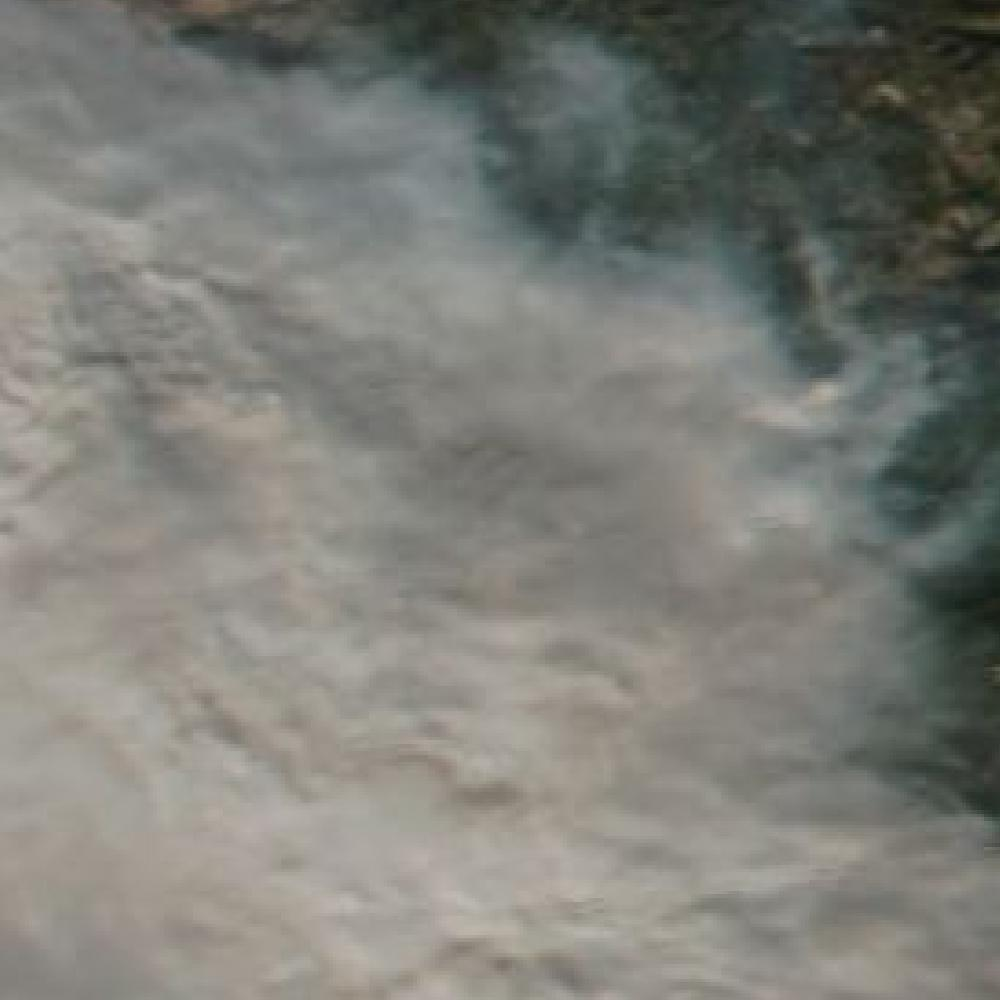
\includegraphics[width=\linewidth]{figuras/camp_color.jpg}
  \caption{Color verdadero: lo que vería el ojo.}
\end{subfigure}\hfill
\begin{subfigure}{0.32\textwidth}
  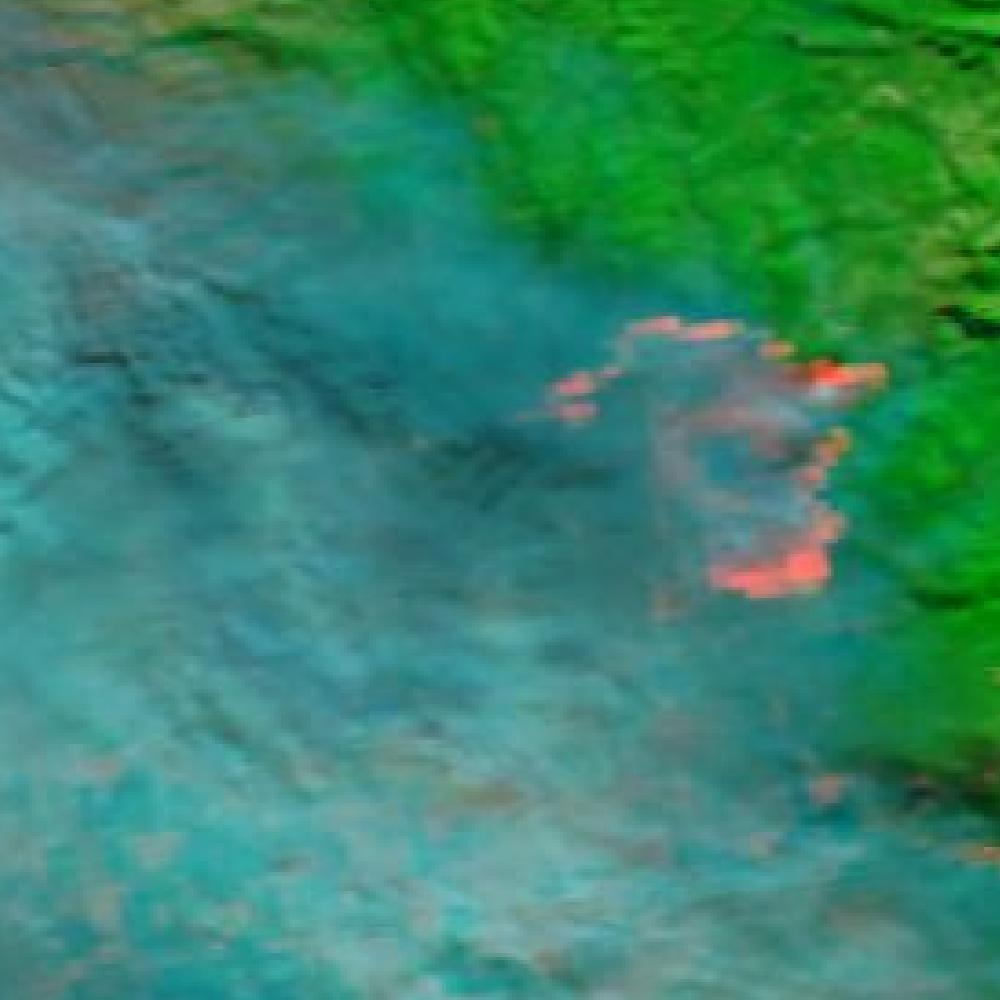
\includegraphics[width=\linewidth]{figuras/camp_falso.jpg}
  \caption{Falso color con infrarrojo de onda corta.}
\end{subfigure}\hfill
\begin{subfigure}{0.32\textwidth}
  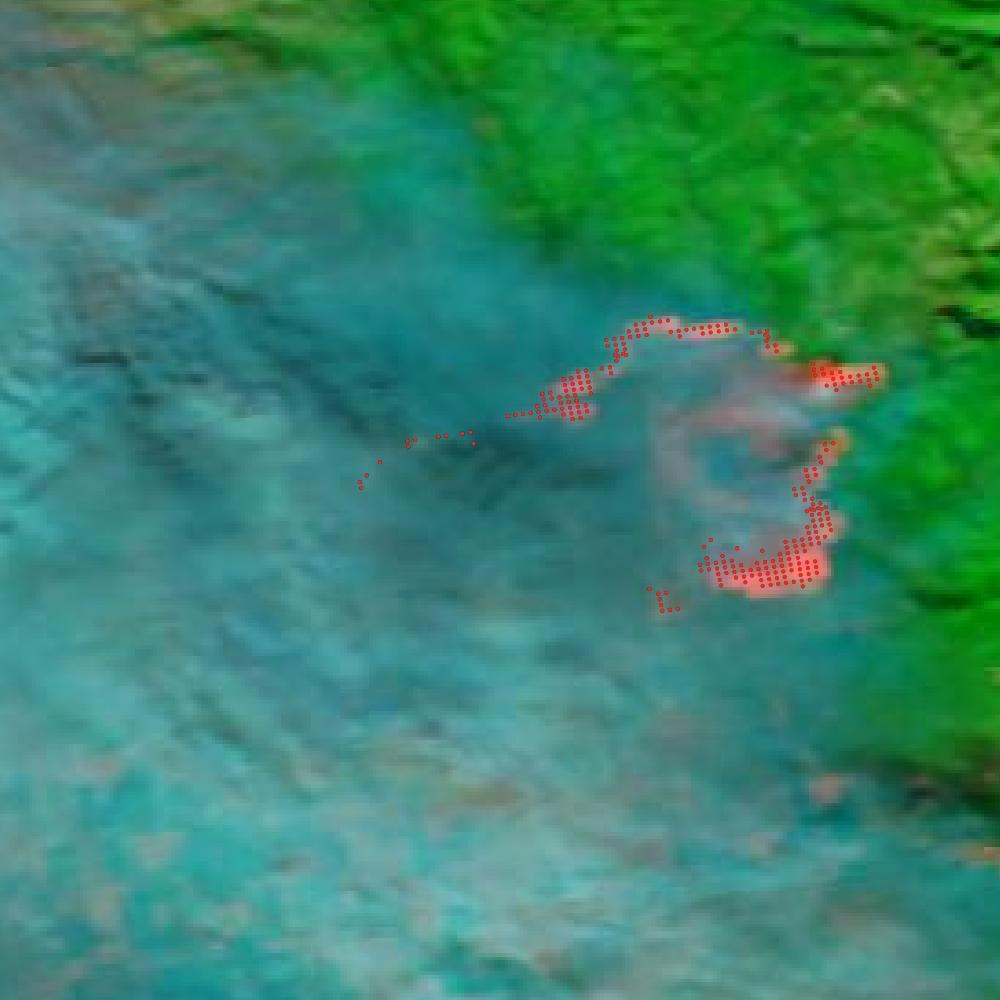
\includegraphics[width=\linewidth]{figuras/camp_focos.jpg}
  \caption{La misma imagen con los focos de 375~m.}
\end{subfigure}

\medskip
\begin{tikzpicture}
  \node[inner sep=0,anchor=south west] (z) at (0,0) {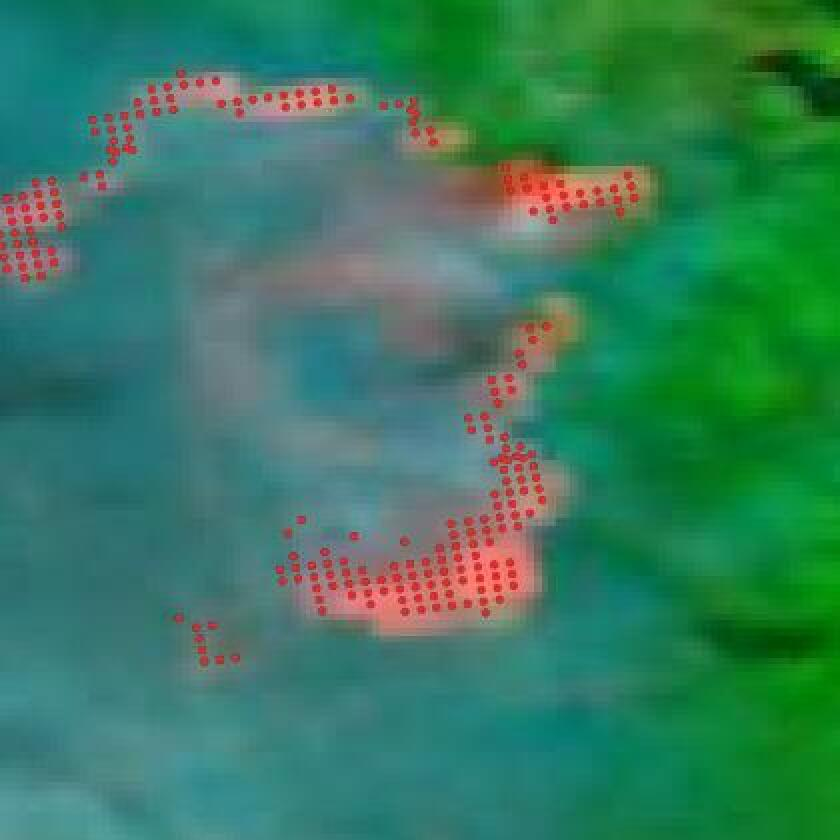
\includegraphics[width=0.5\textwidth]{figuras/camp_zoom.jpg}};
  \node[anchor=west,text width=0.42\textwidth,align=left,font=\small] at ($(z.east)+(0.5,0)$) {%
    \textbf{(d) Ampliación del panel (c).}\\[4pt]
    Cada punto rojo es un foco: el centro de un píxel clasificado como fuego.\\[4pt]
    Los puntos forman una \textbf{rejilla regular}. Esa rejilla no es la forma del incendio: es
    la cuadrícula de píxeles del sensor.\\[4pt]
    El frente continuo de llamas (en naranja brillante) queda convertido en una colección de
    puntos sueltos.};
\end{tikzpicture}
\caption{Un incendio real y sus focos de calor: \emph{Camp Fire}, California, 9 de noviembre de
2018. Imágenes de VIIRS/Suomi NPP obtenidas de NASA Worldview: (a) reflectancia corregida en
color verdadero; (b) combinación de bandas M11--I2--I1; (c) y (d) la misma combinación con la
capa de anomalías térmicas de 375~m.}
\label{fig:camp}
\end{figure}

Los cuatro paneles enseñan cosas distintas.

\textbf{(a) En el visible solo se ve humo.} Una columna densa cubre casi todo el recuadro y
oculta por completo dónde están las llamas.

\textbf{(b) En el infrarrojo se ve el fuego.} Esta combinación asigna al color rojo una banda
del infrarrojo de onda corta (2,25~\um), en la que las superficies muy calientes emiten con
fuerza y que el humo deja pasar. El frente activo aparece como un anillo naranja brillante, el
bosque sano en verde y el humo en tonos azulados y translúcidos. Es una comprobación visual de
lo que explicará el capítulo~\ref{cap:atmosfera}: el infrarrojo atraviesa el humo.

\textbf{(c) y (d) Los focos son la versión digital de ese anillo.} Cada píxel de 375~m del
frente que superó las pruebas del algoritmo se convierte en un punto. En la ampliación se
aprecia que los puntos están alineados en filas y columnas: son centros de píxeles, no
posiciones de llamas.

Este único incendio produjo, en esta sola pasada, un gran número de focos; una quema agrícola
produce uno o ninguno. Quien cuente focos sin pensar en esto estará midiendo sobre todo el
tamaño de los incendios más grandes, y casi nada de los pequeños.

\section{Dos familias de sensores}

Los focos de calor que distribuye la NASA provienen de dos instrumentos.

\termino{MODIS} (\emph{Moderate Resolution Imaging Spectroradiometer}) vuela en dos satélites:
Terra, lanzado a fines de 1999, y Aqua, lanzado en 2002. Su registro de focos empieza en
noviembre de 2000 y es el más largo que existe con cobertura global diaria. Sus píxeles de
fuego miden 1 km en el punto situado justo debajo del satélite.

\termino{VIIRS} (\emph{Visible Infrared Imaging Radiometer Suite}) es su sucesor. Vuela en el
satélite Suomi NPP desde fines de 2011, en NOAA-20 desde fines de 2017 y en NOAA-21 desde fines
de 2022. Su producto principal de focos usa píxeles de 375 m.

La figura~\ref{fig:cronologia} resume el solape disponible. La continuidad exige enlazar
sensores y plataformas, y revisar cambios de procesamiento y hora de paso. Las fechas
se refieren al archivo de focos, no necesariamente al lanzamiento del satélite.

\begin{figure}[ht]
\centering
\begin{tikzpicture}[x=0.43cm,y=0.65cm]
  \draw[->,thick] (0,0)--(28.5,0);
  \foreach \a in {2000,2004,2008,2012,2016,2020,2024}{
    \pgfmathsetmacro{\x}{\a-2000}
    \draw (\x,.12)--(\x,-.12) node[below,font=\footnotesize]{\a};
  }
  \fill[modis!85] (.85,5) rectangle (26.85,5.6);\node[left,font=\small] at (.6,5.3){Terra};
  \fill[modis!60] (2.5,4) rectangle (26.85,4.6);\node[left,font=\small] at (.6,4.3){Aqua};
  \fill[viirs!85] (12.05,2.6) rectangle (26.84,3.2);\node[left,font=\small] at (.6,2.9){Suomi NPP};
  \fill[viirs!65] (18.25,1.6) rectangle (26.85,2.2);\node[left,font=\small] at (.6,1.9){NOAA-20};
  \fill[viirs!45] (23.16,.6) rectangle (26.85,1.2);\node[left,font=\small] at (.6,.9){NOAA-21};
  \draw[dashed,ceniza] (26.85,-.2)--(26.85,6);
  \node[font=\footnotesize,anchor=south east] at (26.85,6){consulta: noviembre de 2026};
  \node[font=\footnotesize,align=center] at (19,-1.3){solape entre plataformas:\\base para comparar sus registros};
\end{tikzpicture}
\caption{Cronología del archivo FIRMS, consultada el 9 de noviembre de 2026. Las barras
se cortan en la fecha de consulta y no predicen el fin de las misiones. Suomi NPP cerró
su entrega el 2 de noviembre de 2026; NOAA-21 figura en el archivo desde marzo de 2023.
Se omiten interrupciones internas. Fuentes: NASA FIRMS y NOAA.\fuente{firms-archive}\fuente{noaa-snpp}}
\label{fig:cronologia}
\end{figure}

\section{Por qué no se pueden sumar}

Imagina que quieres responder una pregunta sencilla: \emph{¿está ardiendo más mi región ahora
que hace veinte años?} Lo natural sería contar los focos de cada año y dibujar la serie. Si lo
haces mezclando sensores, obtienes algo parecido a la figura~\ref{fig:salto}: una serie que da
un salto enorme justo cuando entra VIIRS.

\begin{figure}[ht]
\centering
\begin{tikzpicture}
\begin{axis}[width=13cm,height=6.2cm,ybar,bar width=7pt,
  xlabel={Año},ylabel={Focos por año},ymin=0,ymax=5200,
  xtick={2002,2006,2010,2014,2018,2022},x tick label style={/pgf/number format/1000 sep=},
  scaled y ticks=false,y tick label style={/pgf/number format/1000 sep={\,}},
  legend style={at={(0.5,1.03)},anchor=south,font=\small,draw=none,fill=none,legend columns=2,/tikz/every even column/.append style={column sep=10pt}},
  axis lines*=left,ymajorgrids,grid style={ceniza!20}]
\addplot[fill=modis!80,draw=none] coordinates {(2001,820)(2002,910)(2003,1040)(2004,870)(2005,1260)
 (2006,930)(2007,1110)(2008,880)(2009,960)(2010,1320)(2011,900)};
\addplot[fill=viirs!80,draw=none] coordinates {(2012,3650)(2013,3320)(2014,3480)(2015,3900)(2016,4480)
 (2017,3610)(2018,3540)(2019,3820)(2020,4390)(2021,3700)(2022,3950)(2023,4100)(2024,4750)};
\legend{MODIS,VIIRS}
\draw[<-,thick,ceniza] (axis cs:2011.6,2500)--(axis cs:2008.2,3600)
  node[left,font=\small,align=right,text=black]{¿Se cuadruplicó el fuego\\ en un solo año?};
\end{axis}
\end{tikzpicture}
\caption{Lo que ocurre si se cambia de sensor sin corregir (datos ilustrativos). El salto de
2012 no es un cambio en el fuego: es un cambio en el instrumento con que se lo mira.}
\label{fig:salto}
\end{figure}

El salto es un artefacto. VIIRS detecta más focos que MODIS mirando exactamente los mismos
fuegos, por varias razones que el libro irá desarmando una por una:

\begin{itemize}
  \item Sus píxeles son más pequeños, así que un fuego chico destaca más contra su fondo y es
  detectado, mientras que en un píxel grande de MODIS queda diluido
  (capítulos~\ref{cap:radiacion} y~\ref{cap:deteccion}).
  \item Un mismo incendio ocupa más píxeles pequeños que píxeles grandes, de modo que genera
  más focos aunque los dos sensores lo vean entero.
  \item Sus píxeles crecen mucho menos hacia los bordes de la imagen
  (capítulo~\ref{cap:escaneo}).
  \item Su franja de observación es más ancha y no deja huecos entre órbitas cerca del ecuador
  (capítulo~\ref{cap:orbitas}).
  \item El número de satélites en vuelo ha ido cambiando: uno, dos, tres.
\end{itemize}

\begin{intuicion}[Analogía: dos termómetros]
Supón que una estación meteorológica midió la temperatura durante doce años con un termómetro
viejo que marca dos grados de menos, y luego lo cambió por uno nuevo y exacto. Si unes las dos
series tal cual, <<descubres>> un calentamiento brusco de dos grados el día del cambio. Nadie
aceptaría esa conclusión. Lo correcto es tener ambos termómetros funcionando juntos durante un
tiempo, medir cuánto difieren y corregir una de las series. Eso mismo, con focos en lugar de
grados, es armonizar.
\end{intuicion}

\section{Qué significa armonizar}

\begin{definicion}{armonización}
Armonizar dos registros es transformarlos para que midan la misma cantidad en la misma escala,
de modo que las diferencias que queden entre ellos reflejen cambios del fenómeno observado y no
diferencias entre instrumentos.
\end{definicion}

La armonización es posible gracias al periodo de solape de la figura~\ref{fig:cronologia}.
Desde 2012 ambos sensores observan los mismos lugares, muchas veces con pocos minutos de
diferencia. Esos años permiten \emph{aprender} la relación entre lo que ve uno y lo que ve el
otro, y aplicarla después a los años en que solo existe uno de los dos.

Hay tres preguntas que cualquier método de armonización debe responder, y el libro dedica un
capítulo a cada una:

\begin{enumerate}
  \item \textbf{¿Qué se cuenta?} No es obvio que la unidad correcta sea <<un foco>>. Puede ser
  más robusto contar <<días con fuego en una celda>> (capítulo~\ref{cap:armonizacion}).
  \item \textbf{¿Cómo se relacionan los dos sensores?} Un factor constante, una recta, una
  relación distinta por región y por mes (capítulos~\ref{cap:estadistica}
  y~\ref{cap:armonizacion}).
  \item \textbf{¿Cuánto confiar en el resultado?} Toda corrección tiene incertidumbre y hay que
  saber medirla y mostrarla (capítulo~\ref{cap:estadistica}).
\end{enumerate}

\section{El calendario de quemas}

El producto final que pide el reto no es la serie armonizada en sí, sino una forma de leerla.

\begin{definicion}{calendario de quemas}
Un calendario de quemas es un resumen, para un área elegida, de \textbf{cuándo} arde a lo largo
del año: en qué semanas o meses se concentra históricamente la actividad, cuánta es normal en
cada época y qué periodos concretos se salieron de lo normal.
\end{definicion}

La figura~\ref{fig:calendario-intro} muestra una de sus formas más habituales: una matriz con
los años en un eje y los meses en el otro, coloreada según la actividad. De un vistazo se
reconocen la temporada (la banda vertical más oscura) y los años excepcionales (las filas que
destacan). El capítulo~\ref{cap:calendario} explica cómo se construye y cómo se definen con
rigor <<normal>> y <<excepcional>>.

\begin{figure}[ht]
\centering
\begin{tikzpicture}
\begin{axis}[width=13cm,height=6.7cm,xmin=.5,xmax=12.5,ymin=-.5,ymax=11.5,y dir=reverse,
 xtick={1,...,12},xticklabels={E,F,M,A,M,J,J,A,S,O,N,D},
 ytick={0,2,4,6,8,10,11},yticklabels={2013,2015,2017,2019,2021,2023,2024},
 colormap={peruintro}{color(0cm)=(white);color(1cm)=(brasaClaro);color(2cm)=(fuego)},
 colorbar,colorbar style={ylabel={Celdas-día},scaled ticks=false,tick label style={font=\scriptsize}}]
\addplot[matrix plot*,mesh/cols=12,point meta=explicit,draw=white,line width=.2pt]
 table[x=mes,y=fila,meta=actividad,col sep=comma]{datos/peru_calendario.csv};
\end{axis}
\end{tikzpicture}
\caption{Calendario con \textbf{datos reales de Perú}: VIIRS/Suomi NPP, 2013--2024,
solo detecciones diurnas tipo 0 y de confianza nominal/alta, agrupadas por celda de
$0{,}05^\circ$ y día. Fuente: NASA FIRMS; cálculo propio. Los filtros, las limitaciones
y la comparación estacional se desarrollan en el capítulo~\ref{cap:calendario}.}
\label{fig:calendario-intro}
\end{figure}

\section{El mapa del libro}

La figura~\ref{fig:mapa} resume el camino completo, desde las llamas hasta el número que ve el
usuario. Cada flecha es una transformación que introduce supuestos y errores, y cada una se
estudia en un capítulo. Entender la cadena entera es lo que permite decidir con criterio en el
último eslabón.

\begin{figure}[ht]
\centering
\begin{tikzpicture}[node distance=5mm and 7mm]
  \node[caja,fill=fuegoClaro] (a) {Fuego\\ en el suelo};
  \node[caja,right=of a,fill=brasaClaro] (b) {Radiación\\ infrarroja};
  \node[caja,right=of b,fill=cieloClaro] (c) {Atmósfera};
  \node[caja,right=of c,fill=cieloClaro] (d) {Sensor\\ en órbita};
  \node[caja,right=of d,fill=violetaClaro] (e) {Píxel y\\ algoritmo};
  \node[caja,below=12mm of e,fill=violetaClaro] (f) {Foco de calor\\ (FIRMS)};
  \node[caja,left=of f,fill=bosqueClaro] (g) {Conteo en\\ celdas y días};
  \node[caja,left=of g,fill=bosqueClaro] (h) {Serie\\ armonizada};
  \node[caja,left=of h,fill=bosqueClaro] (i) {Calendario\\ y anomalías};
  \node[caja,left=of i,fill=white] (j) {Decisión\\ del usuario};
  \draw[flujo] (a)--(b); \draw[flujo] (b)--(c); \draw[flujo] (c)--(d); \draw[flujo] (d)--(e);
  \draw[flujo] (e)--(f); \draw[flujo] (f)--(g); \draw[flujo] (g)--(h); \draw[flujo] (h)--(i); \draw[flujo] (i)--(j);
  \node[font=\footnotesize,ceniza,above=1mm of b] {cap.~\ref{cap:radiacion}};
  \node[font=\footnotesize,ceniza,above=1mm of c] {cap.~\ref{cap:atmosfera}};
  \node[font=\footnotesize,ceniza,above=1mm of d] {caps.~\ref{cap:orbitas}--\ref{cap:modisviirs}};
  \node[font=\footnotesize,ceniza,above=1mm of e] {caps.~\ref{cap:deteccion}--\ref{cap:errores}};
  \node[font=\footnotesize,ceniza,below=1mm of f] {cap.~\ref{cap:firms}};
  \node[font=\footnotesize,ceniza,below=1mm of g] {caps.~\ref{cap:armonizacion},~\ref{cap:aplicacion}};
  \node[font=\footnotesize,ceniza,below=1mm of h] {caps.~\ref{cap:estadistica},~\ref{cap:armonizacion}};
  \node[font=\footnotesize,ceniza,below=1mm of i] {cap.~\ref{cap:calendario}};
\end{tikzpicture}
\caption{La cadena completa, de las llamas a la decisión, y el capítulo que estudia cada
eslabón.}
\label{fig:mapa}
\end{figure}

\resumen

\begin{itemize}
  \item Un \textbf{foco de calor} es un píxel clasificado como <<con fuego>> en el instante de
  la observación. No es un incendio, no marca la posición exacta de las llamas y no registra lo
  que ocurre entre una pasada y la siguiente.
  \item El registro de focos de la NASA proviene de \textbf{MODIS} (desde 2000, píxeles de
  1~km) y de \textbf{VIIRS} (desde 2012, píxeles de 375~m). La continuidad exige enlazar los registros y revisar el estado de cada misión.
  \item VIIRS detecta más focos que MODIS ante los mismos fuegos. Unir las dos series sin
  corregir produce un salto artificial.
  \item \textbf{Armonizar} es volver comparables los dos registros usando el periodo en que
  ambos sensores observan a la vez.
  \item El \textbf{calendario de quemas} resume cuándo arde un área a lo largo del año, qué es
  normal y qué fue anómalo.
\end{itemize}

\ejercicios

\begin{enumerate}
  \item Explica con un ejemplo propio por qué <<más focos>> no implica necesariamente <<más
  incendios>>, y por qué tampoco implica <<más superficie quemada>>.
  \item Un sensor tiene píxeles de 1~km y otro de 375~m. ¿Cuántos píxeles del segundo caben en
  uno del primero? Si un frente de fuego recto de 3~km de largo cruza la imagen, ¿cuántos
  píxeles ocupa aproximadamente en cada sensor?
  \item En la figura~\ref{fig:cronologia}, ¿en qué años hay exactamente un sensor MODIS y
  ninguno VIIRS? ¿En cuáles hay dos MODIS y tres VIIRS? ¿Por qué importa esa diferencia al
  contar focos?
  \item En la analogía de los termómetros, ¿qué papel cumple el periodo en que ambos funcionan
  a la vez? ¿Qué pasaría si el termómetro viejo se hubiera retirado el mismo día en que llegó
  el nuevo?
  \item Propón dos usuarios distintos de un calendario de quemas en Junín y escribe, para cada
  uno, la pregunta concreta que querría responder con la herramienta.
\end{enumerate}
